\documentclass[10pt]{article}

%%\RequirePackage{times}
%%\usepackage[times,hyper]{Rd}
\usepackage[utf8,latin1]{inputenc}
\usepackage[T1]{fontenc}
\usepackage{times}


%%\setlength{\textheight}{9.0in}
%%\setlength{\textwidth}{6.5in}
\setlength{\parindent}{0.0in}
\setlength{\parskip}{0.05in}

%%\oddsidemargin=-0.0in
%%\evensidemargin=-0.0in
%%\topmargin=-0.1in

\RequirePackage{bm}              % standard boldsymbol
\RequirePackage{alltt}           % {verbatim} allowing \..
\RequirePackage{verbatim}        % small example code
\RequirePackage{url}             % set urls
\RequirePackage{textcomp}        % for \textquotesingle etc

\usepackage{setspace}


\addtolength{\textheight}{12mm}
\addtolength{\topmargin}{-9mm}   % still fits on US paper
\addtolength{\textwidth}{24mm}   % still fits on US paper
\setlength{\oddsidemargin}{10mm}
\setlength{\evensidemargin}{\oddsidemargin}


\RequirePackage{graphicx}
\usepackage{fancybox}
\usepackage{framed,color}

%%\usepackage{sas.tex}
\RequirePackage[T1]{fontenc}
\RequirePackage{geometry}
\RequirePackage{longtable}
\RequirePackage{times}
\RequirePackage{fancyvrb}
\RequirePackage{array}
%%\RequirePackage{hyperref}
\RequirePackage{graphicx}
\RequirePackage{ifthen}
\RequirePackage{ifpdf}


%%\pagestyle{empty}

\renewcommand{\baselinestretch}{1.3}

\title{Implementing Longitudinal Targeted Minimum Loss Based Estimation (TMLE) for Randomized Trials in SAS and R}
%\date{July 2017}
\author{Aidan McDermott, Elizabeth Colantuoni, Michael Rosenblum}
\begin{document}

\maketitle

\setlength{\abovedisplayskip}{2pt}
\setlength{\belowdisplayskip}{2pt}

\section*{Introduction}

In a repeated measures clinical trial groups of individuals are followed over time with outcome measures taken from each individual at fixed time-points.  Often the focus of the trial is to compare the outcome means in two or more groups at some pre-specified time after enrollment.  Unfortunately, data are not always available for each individual at each time-point.  This can occur for a variety of reasons - individuals may discontinue participating in the study, or they may become non-compliant with the study protocol, or the outcome measure is not taken or it falls outside its detectable range, etc.  If such missingness in the data is ignored and an analysis is performed using only those data available at the specified time-points then bias in the estimates and serious errors in the conclusions drawn from the study can result.

The SAS TMLE macro and R TMLE function uses the longitudinal targeted maximum likelihood estimation of van der Laan and Gruber \cite{vanderLaan2012} which builds on ideas from van der Laan and Rubin \cite{vanderLaan2006}, the sequential regression estimators of Robins \cite{Robins1999}; Bang and Robins \cite{Bang2005}, and the general semiparametric efficiency theory of Robins and Rotnitzky \cite{Robins1992}.  Our estimator can be applied to binary, continuous, or ordinal valued outcomes. Our estimates are made under a missing at random (MAR) assumption and we require that missingness in the data should exibit monotonicity, that is, if an individual is missing data at a time-point then data for that individual should be missing at all subsequent time-points.

\section*{The Data}

The input dataset should be in what is referred to as ``wide'' format. That is, the data from one individual forms a single observation (row) of the dataset.  A variable is used to identify the two groups of interest; this variable should be numeric and take two values, $0$ and $1$.  For example, an input dataset might contain a variable $trt$ to indicate treatment group.  The variable $Y1$ denotes the outcome measured at baseline and variables $Y2$, $Y3$, $Y4$, and $Y5$, hold the outcomes measured at timepoint 2 throught timepoint 5, defining the $NT$ post-baseline assessments.  The input dataset might also contain variables containing values obtained at baseline or at some other time during the study.  In this example we include just two baseline variables $male$ and $age$.
\vspace{0.1in}

\hspace{0.6in}\begin{minipage}[t]{6.8in}
{\renewcommand{\baselinestretch}{1.1}\selectfont%
\begin{minipage}[t]{5.6in}
{\normalsize \em Table 1:  Some observations from the TMLEExample1 dataset.}
\end{minipage}}\vspace{-0.01in}

{\renewcommand{\baselinestretch}{1.1}\selectfont\normalsize\selectfont%
\begin{tabular}{|r|l|r|r|r|r|r|r|r|r|}\hline
\em    Obs & \em    pid & \em    male & \em    age & \em    trt & \em    y1 & \em    y2 & \em    y3 & \em    y4 & \em    y5\\\hline
\em      1 &    ID$-$000259 &    0 &    33 &    0 &    75 &    76 &    69 &    62 &     .\\\hline
\em      4 &    ID$-$010448 &    0 &    35 &    1 &    91 &    93 &    89 &    87 &    83\\\hline
\em      5 &    ID$-$010610 &    1 &    53 &    1 &    72 &    67 &     . &     . &     .\\\hline
\em      7 &    ID$-$011370 &    0 &    49 &    0 &    87 &    90 &    93 &    91 &    98\\\hline
\em     11 &    ID$-$018615 &    1 &    34 &    0 &    81 &     . &     . &     . &     .\\\hline
\em     14 &    ID$-$021971 &    0 &    22 &    0 &    98 &    92 &    95 &    91 &    89\\\hline
\em     16 &    ID$-$022623 &    1 &    24 &    1 &    95 &    97 &    94 &    91 &    94\\\hline
\em     17 &    ID$-$023355 &    0 &    45 &    0 &    74 &    76 &    73 &    74 &    63\\\hline
\end{tabular}
}
\end{minipage}
\vspace{0.3in}

Notice that in this instance three individuals have missing data (observations numbers 1, 5, and 11).  In general, there may be many more variables representing baseline measures and time-varying measures.

\section*{Inputs}

\subsection*{Model specifications}

In order to implement TMLE, three types of models need to be specified.  Potentially two of these model types (dropout and outcome) may require a different model specificaation at each timepoint.  In order to reduce the number of models that the user need specify, three mechanisms are available to specify the models.
\begin{itemize}
\item A {\bf treatment} model.
      This is a logistic model where the dependent variable is the treatment indicator ({\em trt}) in the examples.  The independent variables in the treatment model should be chosen from among the baseline variables.  Only one treatment model need be specified.
\item The {\bf dropout} models.
      For each timepoint $t=1$, $2$, \ldots, $NT - 1$ a logistic model is specified where the dependent variable is an indicator of dropout at time $t+1$ (i.e. the patient is observed at time $t$ but not at time $t+1$).  This dependent variable can also be viewed as an indicator that an individual is last observed at time $t$.  Although the dropout model may vary from timepoint to timepoint you can specify a default model at each timepoint using the {\em dropoutModel} parameter in the TMLE macro call.  Typically this is used to specify baseline variables that should appear in all dropout models.   For example, if you wish to specify that the variables {\em male} and {\em age} should be included all dropout models then specify {\em dropoutModel = male age} in the TMLE macro call . 
%% The dropout models are specified in two parts in order to reduce the amount of typing in many situations.

%%  Firstly, baseline variables that are to be included in all dropout models can be given in the {\em dropoutModel} parameter.  For example, if you wish to specify that the baseline variables {\em male} and {\em age should be included all dropout models then specify dropoutModel = male age. 

%% The {\em csdropout = } parameter controls the number o
At a particular timepoint, $t$, the TMLE macro will add to the dropout model one or more outcome variables.  This is controlled by the {\em lagdropout} parameter which has a default of 1.   If the {\em lagdropout} is 1, then the dropout model will contain the most recent outcome variable prior to $t$.  So specifying {\em dropoutModel = male age} and {\em lagdropout = 1} would result in the model 
$$ logit( E[ D_{t} \mid D_{t-1} = 0, male, age ] = \beta_{0,t} + \beta_{1,t} male + \beta_{2,t} age + \beta_{3,t} Y_t,$$ where $D_t$ is the indicator of dropout at time $t+1$ and $D_0 = 0$ for all patients (i.e. all patients are observed at baseline).
Setting {\em dropoutModel = male age} and {\em lagdropout = 2} would result in the models 
$$ logit( E[ D_{t} \mid D_{t-1} = 0, male, age ] = \beta_{0,t} + \beta_{1,t} male + \beta_{2,t} age + \beta_{3,t} Y_t + \beta_{4,t} Y_{t-1}$$
for $t \ge  2$ and  
$$ logit( E[ D_{t} \mid D_{t-1} = 0, male, age ] = \beta_{0,t} + \beta_{1,t} male + \beta_{2,t} age + \beta_{3,t} Y_t$$
for $t = 1$.

The default dropout model in combination with the {\em lagdropout} parameter can handle many common situations.  However they can't handle all situations.  There are two other mechanisms to handle  model specifications.

If the user wishes to use the default dropout model, except at one or more timepoints, then they can give the full specifcation of the model in the {\em dropoutModelT = } parameter.  For example, to override the default specification at timepoint 3, the user might specify {\em dropoutModel3 = male age Y1}.  This would result in the default models at all times except where $t=3$.

Lastly, the dropout models may be given via a dataset.  If the {\em Modeldata = Models} parameter is set and the Models dataset contains:
%%\vspace{0.1in}

{\ }\hspace{1in}\begin{minipage}[t]{4in}
\begin{spacing}{1.04}
\begin{tabular}[l]{|r|l|l|r|}
   \multicolumn{4}{l}{\normalsize\em The Models Dataset\rule[0.0in]{0.0in}{0.0in}} \\\hline
   {\normalsize\em\em Obs }& 
   {\normalsize\em\em modeltype}&
   {\normalsize\em\em rhs}&
   {\normalsize\em\em tpt}
\\\hline
 1  &    dropout &    male age y1        &  1 \\
 2  &    dropout &    male age aux1 y2   &  2 \\ 
 3  &    dropout &    male age y3        &  3 \\
 4  &    dropout &    male age aux2 y4   &  4 \\
 5  &    outcome &    male age y1        &  2 \\
 6  &    outcome &    male age aux1 y2   &  3 \\
 7  &    outcome &    male age y3        &  4 \\
 8  &    outcome &    male age aux2 y4   &  5 
\\\hline
\end{tabular}
\end{spacing}
\end{minipage}

then the four observations where modeltype = ``dropout'' constitute the four dropout models.

The dropout model at timepoint $t$ is defined using the order:
\begin{itemize}
 \item[{1.}] If a dataset is specified in the {\em Modeldata} parameter which contains an observation with modeltype = ``dropout'' and $tpt = t$, then the model at time $t$ is defined by the variable {\em rhs} in the dataset.
 \item[{2.}] If no dataset is given in the {\em Modeldata} parameter or if no observation in that dataset has modeltype = ``dropout'' and $tpt = t$, and if the {\em dropoutModelT} parameter is set where {\em T} is $t$, then the dropout model at time $t$ is given by the value of {\em dropoutModelT}.
 \item[{3.}] If neither conditions {1.} or {2.} are met then the dropout model at time $t$ is defined by the default {\em dropoutModel} parameter.
\end{itemize}

\item The {\bf outcome} models.
      At timepoint $t = NT+1$ a model is specified where the dependent variable is the outcome at time $NT+1$ and the independent variables are variables available at time $NT+1$.  In addition, for each timepoint $t=2, 3,$ \ldots, $NT$ a model is specified where the dependent variable is the predicted outcome at time $t$ and the indpendent variables are variables available at time $t$.  The outcome model will vary from timepoint to timepoint.  You can specify a default model at each timepoint using the {\em outcomeModel} parameter in the TMLE macro call.  Typically this is used to specify baseline variables that should appear in all outcome models.   For example, if you wish to specify that the variables {\em male} and {\em age} be included all outcome models, then set {\em outcomeModel = male age} in the TMLE macro call . 

At a particular timepoint, $t$, the TMLE macro will add to the outcome model one or more independent outcome variables.  By default TMLE will add the outcome variable at the previous timepoint to the model.   Thus the model would be
$$ E[ Y_{t} \mid D_{t-1} = 0, male, age, Y_{t-1} ] = \gamma_{0,t} + \gamma_{1,t} male + \gamma_{2,t} age + \gamma_{2,t} Y_{t-1} $$ for $t = NT+1$, and   
$$ E[ P_{t} \mid D_{t-1} = 0, male, age, Y_{t-1} ] = \gamma_{0,t} + \gamma_{1,t} male + \gamma_{2,t} age + \gamma_{3,t} Y_{t-1} $$
for $t = 2,3, \ldots, NT$, where $P_{t}$ denotes the predicted value of $Y_t$ based on the fit of the outcome model at time $t+1$.

Setting {\em outcomeModel = male age} and {\em lagoutcome = 2} would result in the models 
$$ E[ Y_{t} \mid D_{t-1} = 0, male, age, Y_{t-1}, Y_{t-2} ] = \gamma_{0,t} + \gamma_{1,t} male + \gamma_{2,t} age + \gamma_{3,t} Y_{t-1} + \gamma_{4,t} Y_{t-2}$$ for $t = NT+1$, and  
$$ E[ P_{t} \mid D_{t-1} = 0, male, age, Y_{t-1}, Y_{t-2} ] = \gamma_{0,t} + \gamma_{1,t} male + \gamma_{2,t} age + \gamma_{3,t} Y_{t-1} + \gamma_{4,t} Y_{t-2}$$ for all times $t = 3, \ldots, NT$ and
$$ E[ P_{t} \mid D_{t-1} = 0, male, age, Y_{t-1} ] = \gamma_{0,t} + \gamma_{1,t} male + \gamma_{2,t} age + \gamma_{3,t} Y_{t-1}$$
at time $t = 2$.

If the user wishes to use the default outcome model, except at one or more timepoints, then they can give the full specifcation of the model at time T in the {\em outcomeModelT = } parameter.  For example, to override the default specification at timepoint 3, the user might specify {\em outcomeModel3 = male age Y1}.  This would result in the default models at all times except where $t=3$.

As with the dropout models the output models may be given via a dataset.  If the {\em Modeldata = Models} parameter is set and the Models dataset contains:
\vspace{0.1in}

{\ }\hspace{1in}\begin{minipage}[t]{4in}
\begin{spacing}{1.1}
\begin{tabular}[l]{|r|l|l|r|}
   \multicolumn{4}{l}{\normalsize\em The Models Dataset\rule[0.0in]{0.0in}{0.0in}} \\\hline
   {\normalsize\em\em Obs }& 
   {\normalsize\em\em modeltype}&
   {\normalsize\em\em rhs}&
   {\normalsize\em\em tpt}
\\\hline
 1  &    dropout &    male age y1        &  1 \\
 2  &    dropout &    male age aux1 y2   &  2 \\ 
 3  &    dropout &    male age y3        &  3 \\
 4  &    dropout &    male age aux2 y4   &  4 \\
 5  &    outcome &    male age y1        &  2 \\
 6  &    outcome &    male age aux1 y2   &  3 \\
 7  &    outcome &    male age y3        &  4 \\
 8  &    outcome &    male age aux2 y4   &  5 
\\\hline
\end{tabular}
\end{spacing}
\end{minipage}

then the four observations where modeltype = ``outcome'' constitute the four output models.

The output model at timepoint $t$ is defined using the order:
\begin{itemize}
 \item[{1.}] If a dataset is specified in the {\em Modeldata} parameter which contains an observation with modeltype = ``outcome'' and $tpt = t$, then the model at time$t$ is defined by the variable {\em rhs} in the dataset.
 \item[{2.}] If no dataset is given in the {\em Modeldata} parameter or if no observation in that dataset has modeltype = ``outcome'' and $tpt = t$, and if the {\em outcomeModelT} parameter is set where {\em T} is $t$, then the outcome model at time $t$ is given by the value of {\em outcomeModelT}.
 \item[{3.}] If neither conditions {1.} or {2.} are met then the outcome model at time $t$ is defined by the default {\em outcomeModel} parameter.
\end{itemize}
\end{itemize}
\newpage
\subsection*{Input parameters}

The following parameters are used in the SAS TMLE macro and R TMLE function:

{\ \ \hspace{0.0in}}
\begin{minipage}[t]{6.2in}
\begin{flushleft}
\small
\renewcommand{\arraystretch}{1.2}
\begin{spacing}{1.1}
\begin{tabular}[l]{|p{1.3in}|p{4.6in}|}
   \multicolumn{2}{l}{\normalsize\em Input and output dataset parameters\rule[0.0in]{0.0in}{0.0in}} \\\hline
   {\normalsize\em\em Parameter }& 
   {\normalsize\em\em Description}
\\\hline
   data =            &  The input dataset  
\\\hline
   out =             &  The output dataset
\\\hline
   outtab =          &  An output dataset suitable for printing
\\\hline
   convgData =       &  Dataset giving the convergence status for each model
\\\hline
   convgSummary =    &  A dataset with summary of convergence status 
\\\hline
   \multicolumn{2}{l}{\normalsize\em Modeling parameters \rule[0.0in]{0.0in}{0.3in}} \\\hline
   {\normalsize\em\em Parameter }& 
   {\normalsize\em\em Description}
\\\hline
   A =               &  The variable indicating group (0 or 1).  
\\\hline
   treatmentModel =  &  This specifies the treatment model
\\\hline
   dropoutModel =    &  This specifies the default dropout model.  This model is used at all timepoints unless one or more dModel$_t$ parameters are set.
\\\hline
   \begin{minipage}[t]{1.3in}
   dropoutModel1 =,\\
   dropoutModel2 =, \ldots    
   \end{minipage}    &  Optionally specify a dropout model for timepoint $t$.  When given this model overwrites the default dropout model at timepoint $t$. 
\\\hline
   lagdropout =      &  When running a dropout model at time $t$ include the lagged outcome variable as an independent variable to the model for lags $1$, $2$, \ldots $lagoutcome$.  If $t < lagoutcome$ then only lags $1$, \ldots $t-1$ are included in the model.  This argument defaults to the lag argument.
\\\hline
   outcomeModelType = & The outcome models are linear models (outcomeModelType = lm) or logistic models (outcomeModelType = lg).  The Default is outcomeModelType = lm.
\\\hline
   outcomeModel =    &  This specifies the default outcome model. It may be changed at specific timepoints using a oModel$_t$ option.  
\\\hline
   \begin{minipage}[t]{1.3in}
   outcomeModel1 =,\\
   outcomeModel2 =, \ldots
   \end{minipage}    &  Opionally specify an outcome model at timepoint $t$.  When given this overwrites the default outcome model at timepoint $t$.  
\\\hline
   lagoutcome =      &  When running an outcome model at time $t$ include the lagged outcome variable as an independent variable to the model for lags $1$, $2$, \ldots $lagoutcome$.  If $t < lagoutcome$ then only lags $1$, \ldots $t-1$ are included in the model.  This argument defaults to the lag argument.
\\\hline
   lag =             &  When either or both of the lagoutcome and lagdropout arguments are not set then this lag is used.  It defaults to 1.
\\\hline
   ModelData =       &  Opionally names a dataset which contains dropout and outcome models at different timepoints. 
\\\hline
\end{tabular}
\end{spacing}
\end{flushleft}
\end{minipage}

{\ \ \hspace{0.0in}}
\begin{minipage}[t]{6.2in}
\begin{flushleft}
\small
\renewcommand{\arraystretch}{1.2}
\begin{spacing}{1.1}
\begin{tabular}[l]{|p{1.3in}|p{4.6in}|}
   \multicolumn{2}{l}{\normalsize\em Bootstrap parameters \rule[0.0in]{0.0in}{0.3in}} \\\hline
   {\normalsize\em\em Parameter }& 
   {\normalsize\em\em Description}
\\\hline
   nreps =           &  Indicate the number of replicate samples.
\\\hline
   seed =            &  The seed to use for sampling.  
\\\hline
   strata =          &  Stratification variables to use in sampling. The default is to stratify by treatment.   
\\\hline
   \multicolumn{2}{l}{\normalsize\em Other parameters \rule[0.0in]{0.0in}{0.3in}} \\\hline
   {\normalsize\em\em Parameter }& 
   {\normalsize\em\em Description}
\\\hline
   clevels =         &  Confidence interval level.  The default is 95\% confidence intervals.
\\\hline
   cutoff =          &  Value used to trim the weights used to fit the outcome regression models.  The default is 20.
\\\hline
\end{tabular}
\end{spacing}
\end{flushleft}
\end{minipage}

\vspace{0.1in}
\newpage

\section*{Examples}
Consider a clinical trial where patients are randomly assigned to two groups, a control group ($trt = 0$) and a treatment group ($trt = 1$).  A questionaire is scored at baseline and administered up to 4 times after baseline.  Scores on the questionaire lie between 0 and 100 with a score above 50 required at baseline for eligibility into the study.  Only sex ( variable male = 1 if subject is male and 0 otherwise), and age ( in years) were recorded at baseline.  The data are stored in the dataset ``TMLEExample1'' where the variable $Y1$ holds the questionaire scores at baseline and $Y2$, \ldots $Y5$ hold the questionaire scores at subsequent timepoints ($NT = 4$).  Descriptive statistics for the two treatment groups are shown.
\vspace{-0.05in}

\hspace{0.6in}\begin{minipage}[t]{6.8in}
{\renewcommand{\baselinestretch}{1.0}\selectfont%
\begin{minipage}[t]{5.6in}
{\normalsize \em Table 2  Descriptive Statistics for the TMLEExample1 dataset.}
\end{minipage}}\vspace{-0.01in}

{\renewcommand{\baselinestretch}{1.0}\selectfont\normalsize\selectfont%
\begin{tabular}[l]{l@{\hspace{0.45in}}rrr@{\hspace{0.45in}}rrr}\hline
   \multicolumn{1}{c}{~} & 
   \multicolumn{3}{c}{\hspace{-0.45in} \em Control} & 
   \multicolumn{3}{c}{\em Treatment} \\[-0.15in]
   \multicolumn{1}{c}{~} & 
   \multicolumn{3}{c}{\hspace{-0.45in}\rule[0.0in]{1.4in}{0.01in}} & 
   \multicolumn{3}{c}{\hspace{-0.12in}\rule[0.0in]{1.4in}{0.01in}} \\[-0.05in]
   \multicolumn{1}{l}{\em Variable} & 
   \multicolumn{1}{r}{\em N} & 
   \multicolumn{1}{r}{\em Percent} &
   \multicolumn{1}{r}{~} & 
   \multicolumn{1}{r}{\em N} & 
   \multicolumn{1}{r}{\em Percent} &
   \multicolumn{1}{r}{~} 
\\\hline
   Male    &    250  &  49.6       &           &   250  &  50.4     &         \rule[0.0in]{0.0in}{0.2in}
\\[0.05in]
   \multicolumn{1}{c}{~} & 
   \multicolumn{3}{c}{\hspace{-0.45in} \em Control} & 
   \multicolumn{3}{c}{\em Treatment} \\[-0.15in]
   \multicolumn{1}{c}{~} & 
   \multicolumn{3}{c}{\hspace{-0.45in}\rule[0.0in]{1.4in}{0.01in}} & 
   \multicolumn{3}{c}{\hspace{-0.12in}\rule[0.0in]{1.4in}{0.01in}} \\[-0.05in]
   \multicolumn{1}{l}{\em Variable} & 
   \multicolumn{1}{r}{\em N} & 
   \multicolumn{1}{r}{\em Mean} &
   {\em SD} & 
   \multicolumn{1}{r}{\em N } &
   \multicolumn{1}{r}{\em Mean} &
   \multicolumn{1}{r}{\em SD}
\\\hline
\rule[0.0in]{0.0in}{0.2in}Age &     250 &    38.624 &    11.973 &      250 &   39.604 &  12.004 \\[0.05in]
    Y1 &     250 &    85.264 &     8.408 &      250 &   85.672 &   8.350\\
    Y2 &     224 &    83.906 &     8.598 &      231 &   84.719 &   8.976\\
    Y3 &     198 &    82.364 &     8.714 &      205 &   83.741 &   9.246\\
    Y4 &     172 &    80.686 &     9.208 &      179 &   82.715 &  10.129\\
    Y5 &     155 &    78.452 &     9.750 &      155 &   82.045 &  10.416   
\\\hline
\end{tabular}}
\end{minipage}
\vspace{-0.01in}

\subsection*{Implementing TMLE using the SAS TMLE macro}\label{SASexamples}

To start, we consider simple models for the data where only the default model types are used.  The treatment model contains the baseline values including the outcome variable at baseline:
$$ Logit( E[ \mbox{trt} = 1 \mid  \mbox{male, age, } Y_1 ] ) =  \alpha_0 + \alpha_1 age + \alpha_2 male + \alpha_3 Y_1 $$
where we denote the logistic function by $Logit$.

There are 4 dropout models which are indexed by time $t = 1, 2, 3, 4$:
$$ Logit( E[ D_{t} \mid D_{t-1}=0 \mbox{male, age, } Y_t ] ) =  \beta_{0,t} + \beta_{1,t} age + \beta_{2,t} male + \beta_{3,t} Y_t $$
There are 4 outcome models to specify, again, one for each post-baseline timepoint $t = 2, 3, 4, 5$:  The last of these models uses the observed outcome as the dependent variable
\[ E[ Y_5 \mid  \mbox{male, age, } Y_4 ] ) =  \gamma_{0,5} + \gamma_{1,5} age + \gamma_{2,5} Y_4 \]
The other three models have the prediced outcome at time $t$ as the dependent variable:
\[ E[ P_{t} \mid  \mbox{male, age, } Y_{t-1} ] ) =  \gamma_{0,t} + \gamma_{1,t} age + \gamma_{2,t} Y_{t-1} \mbox{\ \hspace{0.5in} where } t=2,3,4 \]
Here we are using the fact that the default lag is 1 and so $Y_t$ is automatically added to the dropout models and $Y_{t-1}$ is automatically added to the outcome models.  Also the default outcome model type is the linear model.
We use 10,000 bootstrap samples to compute confidence intervals.
\newpage
\begin{minipage}{\textwidth}
\renewcommand{\baselinestretch}{1.0}\selectfont%
\begin{minipage}[l]{5.6in}
\normalsize\em%
SAS TMLE macro sample code 1.1 (a simple analysis) 
\end{minipage}\vspace{-0.08in}
\begin{Verbatim}[baselinestretch=1.0, fontsize=\small, frame=single, commandchars=\\\{\}]
 libname data    "Data";

 filename macs "macros";
 options sasautos = ( sasautos macs );

 %tmle(
     data           = data.example1,
     outtab         = tab1,
     nreps          = 10000,
     seed           = 31,
     A              = trt,
     outcomeVars    = y1-y5,
     treatmentModel = male age y1,
     dropoutModel   = male age,
     outcomeModel   = male age);
\end{Verbatim}
\end{minipage}
\vspace{0.2in}

\input{tab1.txt}
\newpage
We rerun this analysis including two lags instead of one in the dropout models.  We do this setting the {\em lagdropout} parameter to 2 as shown in sample code 1.2.
\vspace{0.1in}

\begin{minipage}{\textwidth}
\renewcommand{\baselinestretch}{1.0}\selectfont%
\begin{minipage}[l]{5.6in}
\normalsize\em%
SAS TMLE macro sample code 1.2 ( adding a second lag to the dropout model )
\end{minipage}\vspace{-0.08in}
\begin{Verbatim}[baselinestretch=1.0, fontsize=\small, frame=single, commandchars=\\\{\}]
 %tmle(
     data           = example1,
     outtab         = results.tab2,
     nreps          = 10000,
     seed           = 41,
     A              = trt,
     outcomeVars    = y1-y5,
     treatmentModel = male age y1,
     dropoutModel   = male age,
     outcomeModel   = male age,
     lagdropout     = 2);  
\end{Verbatim}
\end{minipage}
\vspace{0.2in}

\input{tab2.txt}
\newpage
Another model that might be considered in this situation is the change over baseline model.  This means that the baseline value of the outcome should be included in the outcome models. At each time $t$, ($t > 1)$, we include  the outcome at time $t-1$ along with the baseline outcome.  The code is in sample code 1.3.

\vspace{0.1in}

%% * TMLE -- a change over baseline model;

\begin{minipage}{\textwidth}
\renewcommand{\baselinestretch}{1.0}\selectfont%
\begin{minipage}[l]{5.6in}
\normalsize\em%
SAS TMLE macro sample code 1.3 (change over baseline)
\end{minipage}\vspace{-0.08in}
\begin{Verbatim}[baselinestretch=1.0, fontsize=\small, frame=single, commandchars=\\\{\}]
  %tmle(
    data           = example1,
    outtab         = results.tab3,
    nreps          = 10000,
    seed           = 51,
    A              = trt,
    outcomeVars    = y1-y5,
    treatmentModel = male age y1,
    dropoutModel   = male age,
    outcomeModel   = male age y1 );
\end{Verbatim}
\end{minipage}
\vspace{0.2in}

\input{tab3.txt}
\newpage
The questionaire results that we have been looking at here are bounded to lie between 0 and 100.  In order to produce predicted values that always lie in this range, we may choose to rescale the outcome and regard it as a proportion.  In this case we divide the outcome variable by 100 so that it lies between 0 and 1 and set the {\em outcomeModelType} parameter to be lg for logistic regression.
\vspace{0.1in}

\begin{minipage}{\textwidth}
\renewcommand{\baselinestretch}{1.0}\selectfont%
\begin{minipage}[l]{5.6in}
\normalsize\em%
SAS TMLE macro sample code 1.4 (outcome variable is ordered between 0 and 1)
\end{minipage}\vspace{-0.08in}
\begin{Verbatim}[baselinestretch=0.9, fontsize=\small, frame=single, commandchars=\\\{\}]
 data example1;   set data.example1;
   array y[*] y1-y5;
   do i = 1 to 5;
     y[i] =  y[i] / 100;
   end; 

 %tmle( data           = example1,     outtab        = results.Ltab1,
        nreps          = 10000,        seed          = 831,
        A              = trt,          outcomeVars   = y1-y5,
        treatmentModel = male age y1,
        dropoutModel   = male age,
        outcomeModel   = male age,
        outcomeModelType = lg );  
\end{Verbatim}
\end{minipage}
\vspace{0.2in}

\input{tab4.txt}

Notice that although this last analysis had the outcome modeled on the logit scale, all the models are similar to those used in sample code 1.1, and indeed, the results are similar after rescaling (multiplying by 100).

As a final example we add to the dataset two variables ``aux1'' and ``aux2''.  These are the results from a supplementary instrument implemented at time $t=2$ (aux1) and $t=4$ (aux2).  Starting with the default model given in sample code 1.1, we wish to add the aux1 variable to the outcome model for $P_3$ and dropout model for $D_2$ and the variable aux2 to the outcome model for $Y_5$ and dropout model for $D_4$.  There are several ways to do this; we begin by modifying the sample code 1.1 to produce sample code 1.5.
\newpage
\begin{minipage}{\textwidth}
\renewcommand{\baselinestretch}{1.0}\selectfont%
\begin{minipage}[l]{5.6in}
\normalsize\em%
SAS TMLE macro sample code 1.5 (time varying covariates other than outcome)
\end{minipage}\vspace{-0.08in}
\begin{Verbatim}[baselinestretch=1.0, fontsize=\small, frame=single, commandchars=\\\{\}]
 %tmle( 
        data           = data.example2,
        outtab         = results.tab5,
        nreps          = 10000, 
        seed           = 1831,
        A              = trt,
        outcomeVars    = y1-y5,
        treatmentModel = male age y1,
        dropoutModel   = male age,
        outcomeModel   = male age,
        dropoutmodel2  = male age aux1 y2,
        dropoutmodel4  = male age aux2 y4,
        outcomemodel3  = male age aux1 y2,
        outcomemodel5  = male age aux2 y4);
\end{Verbatim}
\end{minipage}
\vspace{0.2in}

\input{tab5.txt}

Another way of specifying the models given in code sample 1.5 is given in 1.6.
\vspace{0.1in}

\begin{minipage}{\textwidth}
\renewcommand{\baselinestretch}{1.0}\selectfont%
\begin{minipage}[l]{5.6in}
\normalsize\em%
SAS TMLE macro sample code 1.6 (code produces the same results as sample code 1.5)
\end{minipage}\vspace{-0.08in}
\begin{Verbatim}[baselinestretch=1.0, fontsize=\small, frame=single, commandchars=\\\{\}]
 data modeldata;
     length modeltype  $12;
     length rhs        $200;
     modeltype = "dropout";  
     tpt = 1;  rhs  = "male age y1";      output;
     tpt = 2;  rhs  = "male age aux1 y2"; output;
     tpt = 3;  rhs  = "male age y3";      output;
     tpt = 4;  rhs  = "male age aux2 y4"; output;
     
     modeltype = "outcome";  
     tpt = 2;  rhs  = "male age y1";      output;
     tpt = 3;  rhs  = "male age aux1 y2"; output;
     tpt = 4;  rhs  = "male age y3";      output;
     tpt = 5;  rhs  = "male age aux2 y4"; output;
 run;
     
 %tmle(
     data           = data.example2,
     outtab         = results.tab6,
     nreps          = 10000,
     seed           = 1831,
     A              = trt,
     outcomeVars    = y1-y5,
     treatmentModel = male age y1,
     modeldata      = modeldata);
\end{Verbatim}
\end{minipage}



\vspace{0.2in}
\subsection*{Implementing TMLE using the R TMLE function}

In this section, we replicate the same analyses conducted in Section~\ref{SASexamples} using the R TMLE function.

To start, we consider simple models for the data where only the default model types are used.  The treatment model contains the baseline values including the outcome variable at baseline:
$$ Logit( E[ \mbox{trt} = 1 \mid  \mbox{male, age, } Y_1 ] ) =  \alpha_0 + \alpha_1 age + \alpha_2 male + \alpha_3 Y_1 $$
where we denote the logistic function by $Logit$.

There are 4 dropout models which are indexed by time $t = 1, 2, 3, 4$:
$$ Logit( E[ D_{t} \mid D_{t-1}=0 \mbox{male, age, } Y_t ] ) =  \beta_{0,t} + \beta_{1,t} age + \beta_{2,t} male + \beta_{3,t} Y_t $$
There are 4 outcome models to specify, again, one for each post-baseline timepoint $t = 2, 3, 4, 5$:  The last of these models uses the observed outcome as the dependent variable
\[ E[ Y_5 \mid  \mbox{male, age, } Y_4 ] ) =  \gamma_{0,5} + \gamma_{1,5} age + \gamma_{2,5} Y_4 \]
The other three models have the prediced outcome at time $t$ as the dependent variable:
\[ E[ P_{t} \mid  \mbox{male, age, } Y_{t-1} ] ) =  \gamma_{0,t} + \gamma_{1,t} age + \gamma_{2,t} Y_{t-1} \mbox{\ \hspace{0.5in} where } t=2,3,4 \]
Here we are using the fact that the default lag is 1 and so $Y_t$ is automatically added to the dropout models and $Y_{t-1}$ is automatically added to the outcome models.  Also the default outcome model type is the linear model.
We use 10,000 bootstrap samples to compute confidence intervals.

\begin{minipage}{\textwidth}
\renewcommand{\baselinestretch}{1.0}\selectfont%
\begin{minipage}[l]{5.6in}
\normalsize\em%
R TMLE function sample code 1.1 (a simple analysis) 
\end{minipage}\vspace{-0.08in}
\begin{Verbatim}[baselinestretch=1.0, fontsize=\small, frame=single, commandchars=\\\{\}]
## 
## Read in the example1 dataset
##
example1 = read.table("example1.csv",sep=",",header=T)
##
## Call the TMLE function
## sample code 1.1
##
example1.1 = TMLE(data=example1,A="trt",
     outcomeVars=c("y1","y2","y3","y4","y5"),
     treatmentModel="male age y1",
     dropoutModel="male age",
     outcomeModel="male age",
     lag=1,nreps=10000,seed=123)
\end{Verbatim}
\end{minipage}
\vspace{0.2in}

\begin{minipage}{\textwidth}
\renewcommand{\baselinestretch}{1.0}\selectfont%
\begin{minipage}[l]{5.6in}
\normalsize\em%
R TMLE function output for sample code 1.1 (a simple analysis) 
\end{minipage}\vspace{-0.08in}
\begin{Verbatim}[baselinestretch=1.0, fontsize=\small, frame=single, commandchars=\\\{\}]
                                 Unadj.est Unadj.var Unadj.LL Unadj.UL
 Control (A = 0)                    78.452     0.610   76.855   79.959
 Treatment (A = 1)                  82.045     0.695   80.415   83.670
 Difference (Treatment - Control)    3.594     1.306    1.378    5.811
                                 TMLE.est TMLE.var TMLE.LL TMLE.UL Rel.Eff
 Control (A = 0)                   74.804    0.650  73.046  76.245   1.065
 Treatment (A = 1)                 77.975    0.652  76.404  79.518   0.938
 Difference (Treatment - Control)   3.172    1.085   1.201   5.320   0.831
\end{Verbatim}
\end{minipage}
\vspace{0.2in}
\newpage
We rerun this analysis including two lags instead of one in the dropout models.  We do this setting the {\em lagdropout} parameter to 2 as shown in sample code 1.2.
\vspace{0.1in}

\begin{minipage}{\textwidth}
\renewcommand{\baselinestretch}{1.0}\selectfont%
\begin{minipage}[l]{5.6in}
\normalsize\em%
R TMLE function sample code 1.2 ( adding a second lag to the dropout model )
\end{minipage}\vspace{-0.08in}
\begin{Verbatim}[baselinestretch=1.0, fontsize=\small, frame=single, commandchars=\\\{\}]
example1.2 = TMLE(data=example1,A="trt",
     outcomeVars=c("y1","y2","y3","y4","y5"),
     treatmentModel="male age y1",
     dropoutModel="male age",
     outcomeModel="male age",
     lagdropout=2,nreps=10000,seed=456)
\end{Verbatim}
\end{minipage}
\vspace{0.2in}

\begin{minipage}{\textwidth}
\renewcommand{\baselinestretch}{1.0}\selectfont%
\begin{minipage}[l]{5.6in}
\normalsize\em%
R TMLE function output sample code 1.2 ( adding a second lag to the dropout model )
\end{minipage}\vspace{-0.08in}
\begin{Verbatim}[baselinestretch=1.0, fontsize=\small, frame=single, commandchars=\\\{\}]
                                 Unadj.est Unadj.var Unadj.LL Unadj.UL
 Control (A = 0)                    78.452     0.615   76.864   79.912
 Treatment (A = 1)                  82.045     0.698   80.353   83.643
 Difference (Treatment - Control)    3.594     1.314    1.331    5.839
                                 TMLE.est TMLE.var TMLE.LL TMLE.UL Rel.Eff
 Control (A = 0)                   74.776    0.667  73.044  76.277   1.083
 Treatment (A = 1)                 77.986    0.640  76.347  79.523   0.918
 Difference (Treatment - Control)   3.209    1.085   1.232   5.309   0.826
\end{Verbatim}
\end{minipage}
\vspace{0.2in}
\newpage
Another model that might be considered in this situation is the change over baseline model.  This means that the baseline value of the outcome should be included in the outcome models. At each time $t$, ($t > 1)$, we include  the outcome at time $t-1$ along with the baseline outcome.  The code is in sample code 1.3.

\vspace{0.1in}

%% * TMLE -- a change over baseline model;

\begin{minipage}{\textwidth}
\renewcommand{\baselinestretch}{1.0}\selectfont%
\begin{minipage}[l]{5.6in}
\normalsize\em%
R TMLE function sample code 1.3 (change over baseline)
\end{minipage}\vspace{-0.08in}
\begin{Verbatim}[baselinestretch=1.0, fontsize=\small, frame=single, commandchars=\\\{\}]
example1.3 = TMLE(data=example1,A="trt",
     outcomeVars=c("y1","y2","y3","y4","y5"),
     treatmentModel="male age y1",
     dropoutModel="male age",
     outcomeModel="male age y1",
     lag=1,nreps=10000,seed=789)
\end{Verbatim}
\end{minipage}
\vspace{0.2in}

\begin{minipage}{\textwidth}
\renewcommand{\baselinestretch}{1.0}\selectfont%
\begin{minipage}[l]{5.6in}
\normalsize\em%
R TMLE function output for sample code 1.3 (change over baseline)
\end{minipage}\vspace{-0.08in}
\begin{Verbatim}[baselinestretch=1.0, fontsize=\small, frame=single, commandchars=\\\{\}]
                                 Unadj.est Unadj.var Unadj.LL Unadj.UL
 Control (A = 0)                    78.452     0.619   76.939   80.027
 Treatment (A = 1)                  82.045     0.691   80.353   83.628
 Difference (Treatment - Control)    3.594     1.311    1.325    5.828
                                 TMLE.est TMLE.var TMLE.LL TMLE.UL Rel.Eff
 Control (A = 0)                   74.733    0.644  72.946  76.164   1.041
 Treatment (A = 1)                 77.943    0.640  76.313  79.431   0.927
 Difference (Treatment - Control)   3.209    1.058   1.270   5.315   0.807
\end{Verbatim}
\end{minipage}
\vspace{0.2in}
\newpage
The questionaire results that we have been looking at here are bounded to lie between 0 and 100.  In order to produce predicted values that always lie in this range, we may choose to rescale the outcome and regard it as a proportion.  In this case we divide the outcome variable by 100 so that it lies between 0 and 1 and set the {\em outcomeModelType} parameter to be lg for logistic regression.
\vspace{0.1in}

\begin{minipage}{\textwidth}
\renewcommand{\baselinestretch}{1.0}\selectfont%
\begin{minipage}[l]{5.6in}
\normalsize\em%
R TMLE function sample code 1.4 (outcome variable is ordered between 0 and 1)
\end{minipage}\vspace{-0.08in}
\begin{Verbatim}[baselinestretch=0.9, fontsize=\small, frame=single, commandchars=\\\{\}]
##
## Scale the outcome measuresments
##
example1.scale = example1
for(i in c("y1","y2","y3","y4","y5")) {
  example1.scale[,i] = example1.scale[,i] / 100
}
##
## Call the TMLE function
##
example1.4 = TMLE(data=example1.scale,A="trt",
     outcomeVars=c("y1","y2","y3","y4","y5"),
     treatmentModel="male age y1",
     dropoutModel="male age",
     outcomeModel="male age",
     lag=1,nreps=10000,seed=1234,outcomeModelType="lg")
\end{Verbatim}
\end{minipage}
\vspace{0.2in}
\begin{minipage}{\textwidth}
\renewcommand{\baselinestretch}{1.0}\selectfont%
\begin{minipage}[l]{5.6in}
\normalsize\em%
R TMLE function output for sample code 1.4 (outcome variable is ordered between 0 and 1)
\end{minipage}\vspace{-0.08in}
\begin{Verbatim}[baselinestretch=0.9, fontsize=\small, frame=single, commandchars=\\\{\}]
                                 Unadj.est Unadj.var Unadj.LL Unadj.UL
 Control (A = 0)                    0.7845     1e-04   0.7694   0.8001
 Treatment (A = 1)                  0.8205     1e-04   0.8038   0.8369
 Difference (Treatment - Control)   0.0359     1e-04   0.0131   0.0580
                                 TMLE.est TMLE.var TMLE.LL TMLE.UL Rel.Eff
 Control (A = 0)                   0.7485    1e-04  0.7322  0.7626   0.990
 Treatment (A = 1)                 0.7801    1e-04  0.7642  0.7967   0.988
 Difference (Treatment - Control)  0.0316    1e-04  0.0123  0.0526   0.821
\end{Verbatim}
\end{minipage}
\vspace{0.2in}

Notice that although this last analysis had the outcome modeled on the logit scale, all the models are similar to those used in sample code 1.1, and indeed, the results are similar after rescaling (multiplying by 100).

As a final example we add to the dataset two variables ``aux1'' and ``aux2''.  These are the results from a supplementary instrument implemented at time $t=2$ (aux1) and $t=4$ (aux2).  Starting with the default model given in sample code 1.1, we wish to add the aux1 variable to the outcome model for $P_3$ and dropout model for $D_2$ and the variable aux2 to the outcome model for $Y_5$ and dropout model for $D_4$.  There are several ways to do this; we begin by modifying the sample code 1.1 to produce sample code 1.5.
\newpage
\begin{minipage}{\textwidth}
\renewcommand{\baselinestretch}{1.0}\selectfont%
\begin{minipage}[l]{5.6in}
\normalsize\em%
R TMLE function sample code 1.5 (time varying covariates other than outcome)
\end{minipage}\vspace{-0.08in}
\begin{Verbatim}[baselinestretch=1.0, fontsize=\small, frame=single, commandchars=\\\{\}]
##
## Read in example2.csv file
##
example2 = read.table("example2.csv",sep=",",header=T)
##
## Call the TMLE function
##
example1.5 = TMLE(data=example2,A="trt",
     outcomeVars=c("y1","y2","y3","y4","y5"),
     treatmentModel="male age y1",
     dropoutModel="male age",
     outcomeModel="male age",
     lag=1,nreps=10000,seed=1773,
     dropoutModel2="male age aux1 y2",dropoutModel4="male age aux2 y4",
     outcomeModel3="male age aux1 y2",outcomeModel5="male age aux2 y4")
\end{Verbatim}
\end{minipage}
\vspace{0.2in}

\begin{minipage}{\textwidth}
\renewcommand{\baselinestretch}{1.0}\selectfont%
\begin{minipage}[l]{5.6in}
\normalsize\em%
R TMLE function output for sample code 1.5 (time varying covariates other than outcome)
\end{minipage}\vspace{-0.08in}
\begin{Verbatim}[baselinestretch=1.0, fontsize=\small, frame=single, commandchars=\\\{\}]
                                Unadj.est Unadj.var Unadj.LL Unadj.UL
 Control (A = 0)                   78.4516    0.6221  76.8893  79.9654
 Treatment (A = 1)                 82.0452    0.6918  80.3544  83.6104
 Difference (Treatment - Control)   3.5935    1.3234   1.3191   5.8382
                                 TMLE.est TMLE.var TMLE.LL TMLE.UL Rel.Eff
 Control (A = 0)                  74.9074   0.6013 73.2820 76.3620   0.967
 Treatment (A = 1)                78.0153   0.6459 76.4003 79.5654   0.934
 Difference (Treatment - Control)  3.1079   1.0464  1.1879  5.2397   0.791
\end{Verbatim}
\end{minipage}
\vspace{0.2in}

Another way of specifying the models given in code sample 1.5 is given in 1.6.  The resulting output is identical
to that displayed above.
\vspace{0.1in}

\begin{minipage}{\textwidth}
\renewcommand{\baselinestretch}{1.0}\selectfont%
\begin{minipage}[l]{5.6in}
\normalsize\em%
R TMLE function sample code 1.6 (code produces the same results as sample code 1.5)
\end{minipage}\vspace{-0.08in}
\begin{Verbatim}[baselinestretch=1.0, fontsize=\small, frame=single, commandchars=\\\{\}]
##
## Read in the ModelData.csv file
##
ModelData = read.table("ModelData.csv",sep=",",header=T)
##
## Call the TMLE function
##
example1.6 = TMLE(data=example2,A="trt",
     outcomeVars=c("y1","y2","y3","y4","y5"),
     treatmentModel="male age y1",
     ModelData=ModelData,lag=1,nreps=10000,seed=1773)
\end{Verbatim}
\end{minipage}

\vspace{0.2in}

\section*{A note on convergence}
The TMLE macro employs three types of model:  the treatment model which is a logistic model, the dropout model which is also logistic and the outcome model which may be either a logistic or a linear model.   These models are run for the main input data and for each of the bootstraps.  There are $NT$ dropout and outcome models fit, respectively.  Given a large number of bootstrap samples, convergence in some models may be problematic.  This is particularly true of the dropout models where insufficient dropout at a given timepoint in a particular bootstrap can cause convergence errors.  

The TMLE macro returns two datasets outlining convergence issues.  The first is requested using the  {\em convgdata = } parameter and lists the convergence status for each model ran. A second dataset requested using the {convgSummary = } parameter summarizes the convergence results.  The variable {\em status} in each dataset gives the returned convergence status from PROC LOGISTIC or PROC GENMOD depending of the model requested.  A status of 0 indicates that the model converged.  All other values may indicate a problem.

Here we list the contents of the convgsummary dataset from sample code 1.1. for the input dataset.  There are 17 models in all and all models converged.
\vspace{0.5in}

\begin{minipage}{\textwidth}
\noindent%
{\renewcommand{\baselinestretch}{1.0}\selectfont
\begin{minipage}[l]{5.6in}
\normalsize\em%
TMLE convergence status for the main dataset from sample code 1.1.\\
\end{minipage}}\vspace{-0.11in}%
 
{\renewcommand{\baselinestretch}{1.25}\selectfont\footnotesize\selectfont\noindent%
\noindent%
\begin{tabular}{|l|l|r|r|r|l|r|}\hline
\em   model & \em    modelType & \em    trt & \em    tpt & \em    Status & \em    convgMessage & \em    n\\\hline
   Dropout &    Logistic &    0 &    1 &            0 &    Convergence criterion (GCONV=1E$-$9) satisfied. &            1\\\hline
   Dropout &    Logistic &    0 &    2 &            0 &    Convergence criterion (GCONV=1E$-$9) satisfied. &            1\\\hline
   Dropout &    Logistic &    0 &    3 &            0 &    Convergence criterion (GCONV=1E$-$9) satisfied. &            1\\\hline
   Dropout &    Logistic &    0 &    4 &            0 &    Convergence criterion (GCONV=1E$-$9) satisfied. &            1\\\hline
   Dropout &    Logistic &    1 &    1 &            0 &    Convergence criterion (GCONV=1E$-$9) satisfied. &            1\\\hline
   Dropout &    Logistic &    1 &    2 &            0 &    Convergence criterion (GCONV=1E$-$9) satisfied. &            1\\\hline
   Dropout &    Logistic &    1 &    3 &            0 &    Convergence criterion (GCONV=1E$-$9) satisfied. &            1\\\hline
   Dropout &    Logistic &    1 &    4 &            0 &    Convergence criterion (GCONV=1E$-$9) satisfied. &            1\\\hline
   Outcome &    Linear &    0 &    1 &            0 &    Algorithm converged. &            1\\\hline
   Outcome &    Linear &    0 &    2 &            0 &    Algorithm converged. &            1\\\hline
   Outcome &    Linear &    0 &    3 &            0 &    Algorithm converged. &            1\\\hline
   Outcome &    Linear &    0 &    4 &            0 &    Algorithm converged. &            1\\\hline
   Outcome &    Linear &    1 &    1 &            0 &    Algorithm converged. &            1\\\hline
   Outcome &    Linear &    1 &    2 &            0 &    Algorithm converged. &            1\\\hline
   Outcome &    Linear &    1 &    3 &            0 &    Algorithm converged. &            1\\\hline
   Outcome &    Linear &    1 &    4 &            0 &    Algorithm converged. &            1\\\hline
   Treatment &    Logistic &    . &    . &            0 &    Convergence criterion (GCONV=1E$-$9) satisfied. &            1\\\hline
\end{tabular}}
\end{minipage}
\newpage
The situation among the bootstrap samples is given here.
\vspace{0.2in}

\begin{minipage}{\textwidth}
\noindent%
\begin{flushleft}
{\renewcommand{\baselinestretch}{1.0}\selectfont
\begin{minipage}[l]{5.6in}
\normalsize\em%
TMLE convergence status for the bootstraps from sample code 1.1.\\
\end{minipage}}\vspace{-0.11in}%
 
\begin{minipage}[l]{5.6in}
{\renewcommand{\baselinestretch}{1.25}\selectfont\footnotesize\selectfont\noindent%
\begin{tabular}{|l|l|r|r|r|l|r|}\hline
\em   model & \em    modelType & \em    trt & \em    tpt & \em    Status & \em    convgMessage & \em    n\\\hline
   Dropout &    Logistic &    0 &    1 &            0 &    Convergence criterion (GCONV=1E$-$9) satisfied. &        9,996\\\hline
   Dropout &    Logistic &    0 &    1 &            1 &    Quasi$-$complete separation of data points detected. &            4\\\hline
   Dropout &    Logistic &    0 &    2 &            0 &    Convergence criterion (GCONV=1E$-$9) satisfied. &       10,000\\\hline
   Dropout &    Logistic &    0 &    3 &            0 &    Convergence criterion (GCONV=1E$-$9) satisfied. &       10,000\\\hline
   Dropout &    Logistic &    0 &    4 &            0 &    Convergence criterion (GCONV=1E$-$9) satisfied. &        9,998\\\hline
   Dropout &    Logistic &    0 &    4 &            1 &    Quasi$-$complete separation of data points detected. &            2\\\hline
   Dropout &    Logistic &    1 &    1 &            0 &    Convergence criterion (GCONV=1E$-$9) satisfied. &        9,992\\\hline
   Dropout &    Logistic &    1 &    1 &            1 &    Quasi$-$complete separation of data points detected. &            8\\\hline
   Dropout &    Logistic &    1 &    2 &            0 &    Convergence criterion (GCONV=1E$-$9) satisfied. &       10,000\\\hline
   Dropout &    Logistic &    1 &    3 &            0 &    Convergence criterion (GCONV=1E$-$9) satisfied. &       10,000\\\hline
   Dropout &    Logistic &    1 &    4 &            0 &    Convergence criterion (GCONV=1E$-$9) satisfied. &       10,000\\\hline
   Outcome &    Linear &    0 &    1 &            0 &    Algorithm converged. &       10,000\\\hline
   Outcome &    Linear &    0 &    2 &            0 &    Algorithm converged. &       10,000\\\hline
   Outcome &    Linear &    0 &    3 &            0 &    Algorithm converged. &       10,000\\\hline
   Outcome &    Linear &    0 &    4 &            0 &    Algorithm converged. &       10,000\\\hline
   Outcome &    Linear &    1 &    1 &            0 &    Algorithm converged. &       10,000\\\hline
   Outcome &    Linear &    1 &    2 &            0 &    Algorithm converged. &       10,000\\\hline
   Outcome &    Linear &    1 &    3 &            0 &    Algorithm converged. &       10,000\\\hline
   Outcome &    Linear &    1 &    4 &            0 &    Algorithm converged. &       10,000\\\hline
   Treatment &    Logistic &    . &    . &            0 &    Convergence criterion (GCONV=1E$-$9) satisfied. &       10,000\\\hline
\end{tabular}}
\end{minipage}
\end{flushleft}
\end{minipage}
\vspace{0.2in}

As can be seen all the the Treatment and Outcome models have converged and most of the Dropout models have converged.  Among the 40,000 Dropout models in treatment 0, 6 did not converge and gave the convergence text associated with ``Quasi$-$complete separation of data points detected.''  Among the 40,000 Dropout models in treatment 1, 8 did not converge and gave the same convergence text.

Complete separation occurs in a logistic model when a linear combination of the independent variables separates the levels of the outcome variable.  This is illustrated in {\em Figure 1} below.  When the values of {\em x} are ``low'' all the values of the outcome variable {\em y} are 0 and when the values of {\em x} are ``high'' all the values of the outcome variable {\em y} are 1.  No data exist between the ``low'' and ``high'' values of {\em x}.  In this situation tThe values of {\em x} discriminate the values of {\em y} very well, but it is not possible to estimate the logistic parameters.  If we were to fit a logistic curve to the data it is clear that in the ``low'' range of {\em x} the fitted curve should be close to 0 and in the ``high'' range the fitted curve should be close to 1, but there is no information in the data to  decide what should happen between the ``low'' and ``high'' values of {\em x}.   Since TMLE only uses fitted values (that is, values in the ``low'' or ``high'' range of {\em x}) differences in the fitted values among these models is not considered important. The logistic procedure will return the last fitted values before it terminates and these are used to produce the weights.
\vspace{0.2in}

\hspace{0.8in}\begin{minipage}[t]{5in}
{\renewcommand{\baselinestretch}{1.0}\selectfont
\hspace{0.4in}\begin{minipage}[t]{4.0in}
{\normalsize \em Figure 1: Quasi-separated outcomes in logistic regression.}
\end{minipage}}\vspace{0.02in}

{
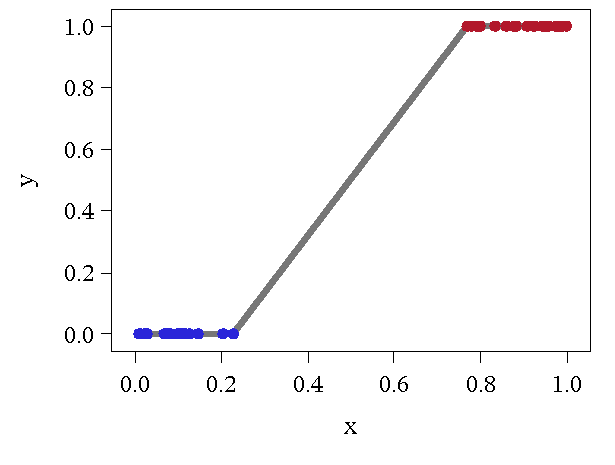
\includegraphics[width=4in]{quasi.pdf}
}
\end{minipage}
\vspace{0.1in}

Another convergence problem can arise. In some bootstraps at some timepoint $t$ no one may dropout of the study.  Under these circumstances the logistic procedure will not run.  TMLE uses the mean value of the dropout indicator to estimate the probability of dropping out at time $t+1$. In this case the status variable is set to 9 and the convgMessage variable is set to ``Not run (mean used)''.

\newpage
\bibliographystyle{plain}
\bibliography{TMLE}{}
\end{document}
